\subsection{Transmission power control}
Protocols in this category try to minimise the power required to transmit
a message. This class of algorithm is akin to a graph optimisation problem,
with the nodes in the MANET represented as nodes in a graph, the power required for
transmitting over a link $p_{ij}$ represented as the cost of a vertex, and the goal
to search the minimum-cost path between two nodes.

\subsubsection{Flow augmentation routing (FAR)}
Flow augmentation routing (FAR)\cite{chang2000energy} finds the routing
path in a (static) network that minimises the sum of link costs in the network,
where the link cost between $i$ and $j$ is defined as \( e_{ij}^{x_{i}}E_{i}^{x_{2}}R_{i}^{-x_{3}}\);
\(e_{ij}\) is the energy cost for the transmission, $E_{i}$ is the initial energy
of the node $i$ and $R_{i}$ is the residue energy of the node. \(x_{1}, x_{2}, x_{3}\)
are weighting factors. As an example, if $x_{1}=x_{2}=x_{3}=0$, then the cost
of each link is 1, and the optimal path is the shortest distance path.

In a static wireless network, $E_{i}$ and $e_{ij}$ are constant, but $R_{i}$
continues to decrease. Thus, the optimal link at one point in time might not be the
optimal link at a different point in time. FAR solves this problem iteratively:
Calculating the optimal path at each step, after updating the residual energy
and link costs.

\subsubsection{Online max-min (OMM)}
\begin{figure*}
\centering
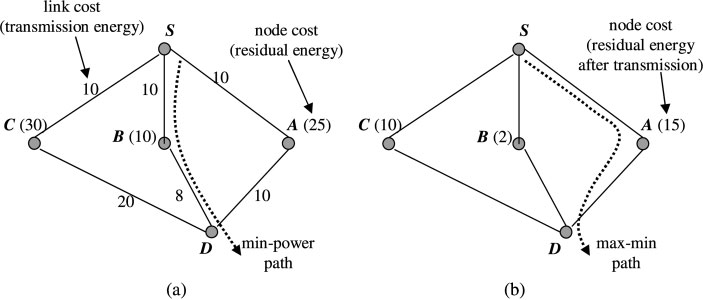
\includegraphics[width=0.7\textwidth]{images/omm}
\caption{Paths in OMM\cite{alotaibi2012survey}}
\label{ommex}
\end{figure*}
\label{omm}
OMM \cite{li2001online} maximises the network lifetime using two metrics:
\begin{enumerate}
  \item \textbf{min-power} - Minimising the overall power
  \item \textbf{max-min} - Maximising the minimum residual power
\end{enumerate}

First OMM calculates the \textit{min-power} path using Dijkstra’s algorithm. Let
the power required by that be $P_{min}$.
Then it determines the \textit{max-min} paths by looking at all paths whose
power do not deviate much from the min-power path, that is, less than $zP_{\min}$
for some $z \ge 1$. It calculates the minimum residual power of all nodes
after the transmission would have taken place, and chooses the path where
that value is largest.

For example, in Figure~\ref{ommex}, we can see that the min-power path from
$S$ to $D$ is $S \to B \to D$ with a value of 18 ($S \to A \to D$ has 20,
$S \to C \to D$ has 30).
It's minimum residual energy will be $2$, as node $B$ needs
$8$ out of the $10$ power units it has.

Looking at the alternate paths, we see that $S \to C \to D$ will have a
minimum residual energy of $30-20=10$ in node $C$, and $S \to A \to D$ will
have a minimum residual energy of $25-10$ in node $A$.
Thus, the max-min path is $S \to A \to D$.

Choosing a good value for $z$ in $zP_{\min}$ is important: For $z=1$, only
the min-power path is considered; for $z \to \inf$, all paths can be
considered. The algorithm starts with a \textit{random} value for $z$, and
then measures the residual energy (\textit{lifetime}) of of the most overloaded node during some
fixed time period. Afterwards, the value of $z$ is increased by a small constant
and the lifetime is measured again. If the lifetime increases, the value of $z$
is increased, otherwise, it is decreased. Because the lifetime is measured
in two distinct time periods, it is assumed that load distribution is roughly
similar, otherwise the results might not be really useful.


\subsubsection{Energy Efficient Routing Protocol in MANET (EERP)}
EERP\cite{main2} is a variation of DSR that stores a minimum energy field
in a route request package, which is set to 100 percent at the beginning. Each
intermediate node will then override the value if its own residual energy rate
is lower than the stored one. The packet is then forwarded if the nodes residual
energy is above a certain threshold.

Once the route requests reach the destinations, the destination picks the route
with the maximum minimum hop energy, that is the \textit{max-min} path. OMM
does something similar, but EERP seems to use the power
levels before the transmission whereas OMM uses the power levels after the
transmission and can also switch to min-power paths.

\subsubsection{Power aware localized routing (PLR)}
PLR\cite{stojmenovic2001power} is a geographical routing protocol, at least
to a certain extend, that tries to minimise the overall power usage. Each node
selects the next hop based on the power required for sending to this node, and
sending from that node indirectly to the destination.

For this, it has to know the locations of the next hops and the location of
the destinations. Based on the locations and the distance between the locations,
it can then estimate the power usage.

For direct connections, this is given in (\ref{eq:plr:p}),
for some constants $a$ and $c$ and some $\alpha \ge 2$ (that is, power usage
is at least growing quadratic in relation to the distance).
\begin{align}\label{eq:plr:p} p(d) := ad^{\alpha} + c \end{align}

For indirect communication between the next hop and the final destination,
the power usage can be calculated as in (\ref{eq:plr:q}), where $n-1$ (\ref{eq:plr:n}) is the optimal number of intermediate nodes\cite{stojmenovic2001power}.
\begin{align}
  \label{eq:plr:q}
   q(d) &:= cn + da \left(\sfrac{a(\alpha - 1)}{c}\right)^{\sfrac{(1-\alpha)}{\alpha}}, \\
   \label{eq:plr:n}
      n &:= d\left(\sfrac{(a(\alpha - 1))}{c}\right)^{\sfrac{1}{\alpha}};
\end{align}

So, given an example like Figure~\ref{plrexample} with a source node $A$, neighbours $N_{1}$, $N_{2}$, and $N_{3}$, and a
destination $D$, $A$ should chose the next hop as the $N_{i}$ for which
$p(|AN_{i}|) + q(|N_{i}D|)$ is minimal.

\begin{figure*}
\centering
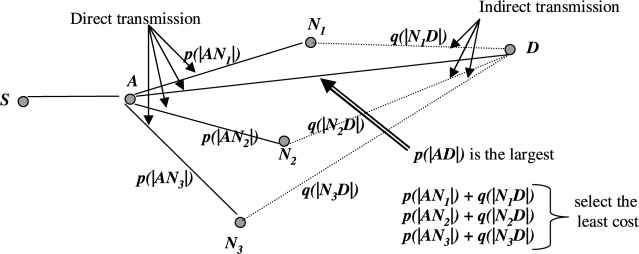
\includegraphics[width=0.7\textwidth]{images/plr-example}
\caption{Selection of next hop in PLR\cite{alotaibi2012survey}}
\label{plrexample}
\end{figure*}

\subsubsection{Minimum energy routing (MER)}
MER\cite{doshi2002demand} modifies the dynamic-source-routing (DSR)\cite{johnson1996dynamic}
and 802.11 MAC algorithms\cite{woesner1998power} with 8 options (table~\ref{tbl:mer-options}) in order to
(1) obtain power information, (2) measure overhead of energy-awareness, and
(3) maintain the minimum power route with mobile nodes.

\begin{table}[tb]
  \begin{tabular}{ll}
    Options & Implementation Level  \\
    \hline
    A: Routing packet-based power control & Routing software/\\ &802.11 firmware \\
    B: Minimum energy routing & Routing software \\
    C: Cache replies off & Routing software \\
    D: Internal cache options & Routing software \\
    E: Multi-hop route discovery & Routing software \\
    F: MAC layer ACK power control & 802.11 firmware \\
    G: Route Maintenance with power sensing & Routing software \\
    G: HMAC-Level snooping and gratious replies & 802.11 firmware \\
  \end{tabular}
  \caption{Options in MER}
  \label{tbl:mer-options}
\end{table}

Option $A$ modifies \textit{route-request} packages of the DSR protocol to
include the power used by the sender, which can the be added to the power
of the receiver to calculate the minimum power required for transmissions
from that sender to it. The value is appended at each intermediate node, and the
destination node then includes it in its \textit{route-reply} header.

The source node than includes this information when it's sending a packet, and
all nodes transmit that package with the controlled power level.

Option F does the same for the MAC layer's ACK packets.

Option $B$ is related to the route cache of the DSR protocol ($C$ and $D$ as well). It
uses the information obtained by option $A$ to select the route that requires
the minimum energy amongst its cached routes.

Option $G$ takes care of adjusting routes when the power transmittion requirements
change because nodes moved.

Option $E$ and $H$ allow nodes not participating in the routing to recommend
alternative, more energy-efficient, routes.
\subsubsection{Local Minimum Energy Dynamic Source Routing Protocol (MEDSR)}
MEDSR\cite{tanque2007minimum} modifies the messages of the DSR protocol to
provide zero-overhead (as in: no extra control messages) energy-aware routing.

MEDSR uses two power levels for route discovery: A low one, and a high one. If
the source does not receive a reply for three route request messages at low
power, it switches to the high power level.

In contrast to other algorithms like MER, it only stores one power level field
in the packets, rather than one power-level per link. That power level is stored
in amended route request and route reply packets.

When a node $C$ receives a route reply from a node $D$, it can estimate the
power level required for transmitting to $D$ by calculating the minimum power
level as in (\ref{eq:medsr:pmin}), where $P_{tx}$ is the transmit power of $D$, $P_{recv}$ the receive power of $C$,
and $P_{th}$ is the threshold power for a successful receive. In 802.11, that's
usually $3.652 \cdot 10^{-10}$ watt.
\begin{align}
  \label{eq:medsr:pmin}
   P_{min} &:= P_{tx} - P_{recv} + P_{th} 
\end{align}
In order to avoid instability of the link, a margin is added,
leading to a modified definition (\ref{eq:medsr:pmin2}) of $P_{min}$.
\begin{align}
  \label{eq:medsr:pmin2}
   P_{min} &:= P_{tx} - P_{recv} + P_{th} + P_{margin}
\end{align}

In addition to the usual tables maintained by DSR, MEDSR also stores a power
table at each node: For each node, the minimum power required to reach it.

\subsubsection{Retransmission-energy aware routing (RAR)}
Transmissions may have link errors which require re-transmitting packets over
a link. A path with many short links might be more efficient than a path with
few long distance links in the absence of link errors, but with link errors,
things might look different, because some packets need to be re-transmitted.

RAR\cite{banerjee2002minimum} introduces a modified cost/power requirement
$P_{i,i+1}$ (\ref{eq:rar:linkcost}) of a link $p_{i,i+1}$ by including the error
rate of that link $e_{i,i+1}$ .
\begin{align}\label{eq:rar:linkcost}
  P_{i,i+1} = \underbrace{p_{i,i+1}}_{\text{original link cost}} \cdot \underbrace{\sfrac{1}{\overbrace{(1-e_{i,i+1})}^{\text{success rate}}}}_{\text{expected number of tries}}
\end{align} 

\subsubsection{Smallest common power (COMPOW)}
Network protocols often require handshaking of some sorts, like acknowledgements
sent to a sender for his packages. Thus, for a MANET to be reliable for those
protocols, for every two nodes, there must be routes in both directions, that
is, some form of bi-directionality.

The smallest common power\cite{narayanaswamy2002power} achieves bi-directionality
of communication in the network.
It does so by maintaining a smallest common transmission power for all nodes,
chosen so that all nodes can communicate with each other. If the power is too
low, some nodes could not reach some others, if it is too high, there might be
many redundant paths. See Figure~\ref{compow:power-choice}.


\begin{figure*}
\centering
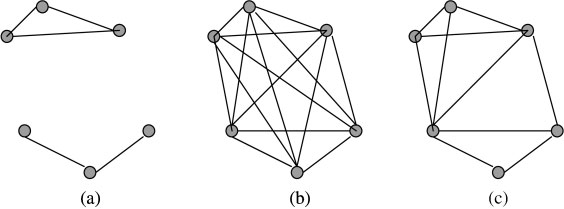
\includegraphics[width=0.7\textwidth]{images/compow-level-choice}
\caption{Power choice in COMPOW: (a) too low, (b) too high, (c) optimal}
\label{compow:power-choice}
\end{figure*}

COMPOW assumes a discrete set of power levels $P_{i}$ and maintains routing
tables ${RT}_{P_{i}}$ containing all nodes reachable from the current one. The
optimal power level $P_{i}$ can be determined as the smallest one for which
$\mid RT_{P_{i}} \mid$ is equal to the number of nodes in the network, by
exchanging the routing tables between nodes.

\subsubsection{PARO}
The PARO Protocol\cite{gomez2003paro} introduces intermediate nodes into a
route, increasing the length of the route, in order to reduce the transmission
power required by each node.
